\documentclass{article}

\usepackage{amsmath}
\usepackage{graphicx}
\usepackage{bbold}


\title{Examination project 14: Inverse iteration method\\ \small Practical Programming and Numerical Methods 2020}
\author{Marco Majland}
\begin{document}
	\maketitle
	\noindent
	The objective of the project is to iteratively calculate the eigenvalue of a given real symmetric matrix, $A$, closest to an input eigenvalue and its associated eigenvector. This is done using the inverse iteration method which is an improvement of the power iteration method. By shifting the matrix equation of the power method, one obtains the inverse iteration method.\\
	Let $\mathbf{A}$ denote a real  symmetric matrix of dimension $n\times n$ and the initial guess of the eigenvalue and eigenvector be $s$ and $\mathbf{u}$ (normalized), respectively. The inverse iteration method is then given by
	\begin{equation}
		(\mathbf{A} - s\mathbb{1})\mathbf{v} = \mathbf{u}
	\end{equation}
	where $\mathbf{v}$ is the refined eigenvector of $\mathbf{A}$. In the implementation of the inverse iteration algorithm, the above linear matrix equation is solved using QR decomposition.
	
	\begin{equation}
		S(x) = \int_{0}^{x}\sin\Big(\frac{\pi t^2}{2}\Big)dt = \sum_{n = 0}^{\infty}(-1)^{n}\frac{x^{4n+3}}{(2n+1)!(4n+3)}
	\end{equation}
	
%	\begin{figure}
%	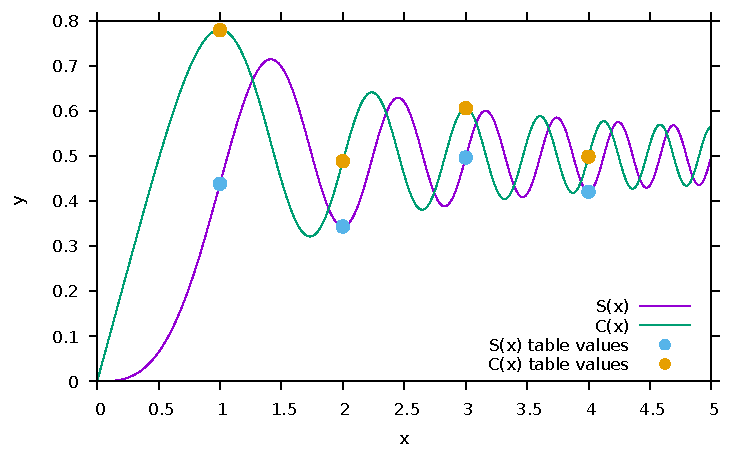
\includegraphics[]{Output.pdf}
%	\caption{Numerical integration of the Fresnel integrals given by equation \ref{eq:Fresnel_integrals} along with the tabulated values given by \%cite{ref1}.}
%	\label{fig:integration}
%	\end{figure}
	
\begin{thebibliography}{9}
	\bibitem{ref1}
	A. Van Wijngaarden and W. L. Scheen,
	\textit{Table of Fresnel integrals},
	The Computation Department of the Mathematical Centre, Amsterdam,
	1949.
\end{thebibliography}
\end{document}